\clearpage{}
\section{Define the stages of a software lifecycle. Describe and compare the
waterfall model, the V model, the spiral model and the agile model of
software development. Discuss the addition of prototyping.}

\subsection{Stages of a software lifecycle}

The software life cycle has the following stages:

\begin{description}
    \item[Requirements analysis and definition]:
    \item[System (architecture) design]:
    \item[Program (detailed) design]:
    \item[Program writing (implementation)]:
    \item[Unit testing]:
    \item[Integration testing]:
    \item[System testing]:
    \item[System delivery]:
    \item[Maintenance]:
\end{description}

\begin{figure}[!ht]
\begin{minipage}{\linewidth}
\begin{minipage}{0.45\linewidth}
\subsection{The waterfall model} The waterfall model was one of the first
models proposed, it is a simple basis for defining more complex models.
It can be used for well understood problems that have stable requirements,
for example if you are at the version 36 of your accounting software with
stable customer needs, this process works pretty well.
% TODO : Integrate text from Thibaut
% This is one of the first models to be proposed. The stages are depicted as cascading from one to another (i.e. one development stage should be completed before the next begins).
%It works for well-understood problems with stable requirements.
%Waterfall model is simple, easy to understand and explain (very high-level view).
%On the other hand, it cannot handle changes (frozen requirements, manufacturing process rather than creative, no iterative activities) and there is a long wait before a final product.

\end{minipage}
\begin{minipage}{0.45\linewidth}
    \centering
    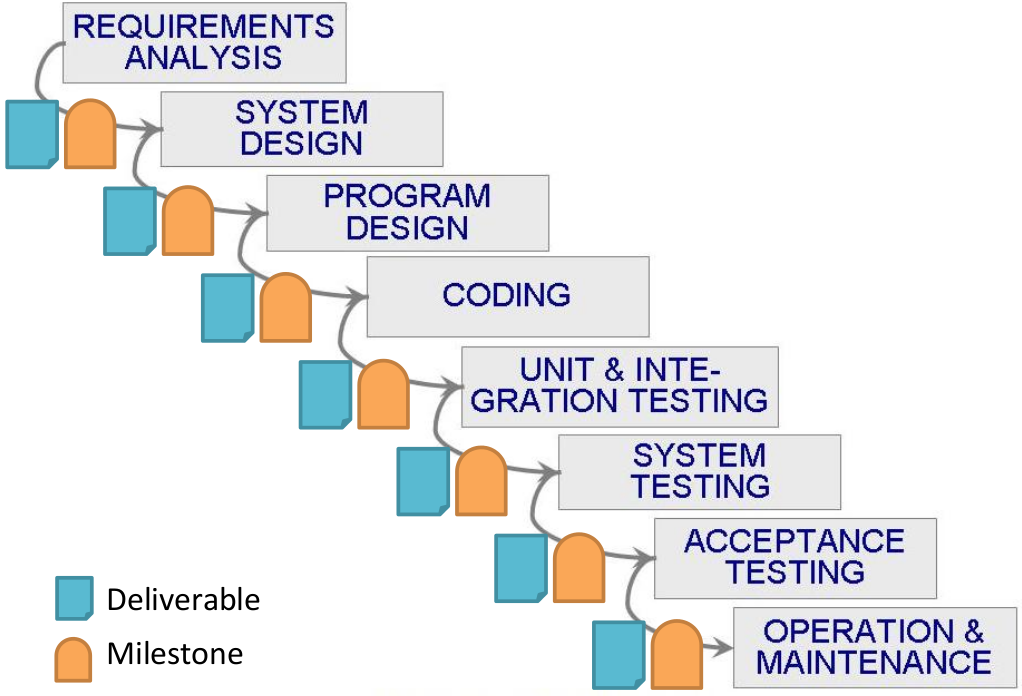
\includegraphics[width=\linewidth]{waterfall_plus.png}
    \caption{Waterfall model lifecycle}
\end{minipage}
\end{minipage}
\end{figure}

\subsection{The V model} The V model is a variation of the waterfall model
that separates it in two phases: \textbf{development} (design) and
\textbf{testing} (V\&V\footnote{Verification and validation}). If one part
of the design wasn't done well, we will discover it during the tests and
we can loop back to this step of the design to restart with a good basis.
% TODO : Integrate text from Thibaut
% This is a variation of the waterfall model that demonstrates how the testing activities are related to analysis and design (development activities). If problems are found, we loop back to the left side of the “V”. In other words, the V model makes more explicit some iterations and reworks that are hidden in the waterfall model.

\begin{figure}[!ht]
    \centering
    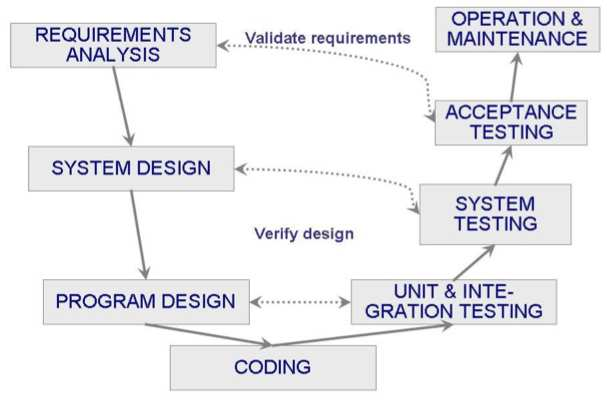
\includegraphics[width=0.8\linewidth]{v_model_2.png}
    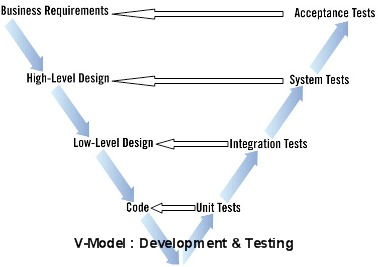
\includegraphics[width=0.8\linewidth]{v_model.png}
    \caption{V model lifecycle}
\end{figure}

\subsection{The spiral model}

This model combines development activities with risk management to minimize and
control risk. It is a sort of iterative development (full system at the very
beginning and then changes functionality of each subsystem with each new
release). \newline

Four basic activites that must occur in each cycle of the spiral model:

\begin{enumerate}
    \item Consider the win conditions of all success-critical stakeholders.
    \item Identify and evaluate alternative approaches for satisfying the win
    conditions.
    \item Identify and resolve risks that stem from the selected approach(es)
    (e.g.\ you can try resolve it, by making a prototype which valid the
    approach).
    \item Obtain approval from all success-critical stakeholders, plus
    commitment to pursue the next cycle.
\end{enumerate}

\begin{figure}[!ht]
    \centering
    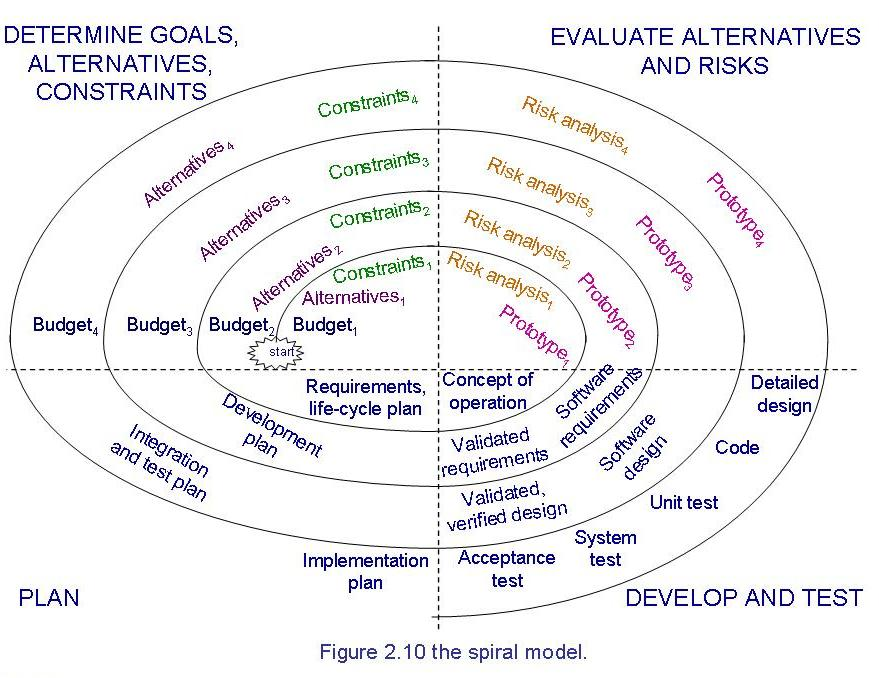
\includegraphics[width=0.8\linewidth]{spiral_model.png}
    \caption{Spiral model lifecycle}
\end{figure}

\subsection{Agile model}

The classical software development process models are rigorous process for
software conception, documentation, development and testing.

The alternative is the agile method that is a flexible process that can adapt to
changing requirements. The overall goal of agile development is to satisfy the
customer by \enquote{early and continuous delivery of valuable software}.

Agile Manifesto:

\begin{itemize}
    \item Value individuals and interactions over processes and tools
    \item Prefer to invest time in producing working software rather than in producing comprehensive documentation
    \item Focus on customer collaboration rather than contract negotiation
    \item Concentrate on responding to change rather than on creating a plan and then following it
\end{itemize}


Examples of agile processes:

\begin{itemize}
    \item Extreme programming (XP)
    \item Crystal
    \item Scrum
\end{itemize}

\subsection{Addition of prototyping}

Prototyping means building a small version of a system (usually with limited
functionality) that can be used to:

\begin{itemize}
    \item Demonstrate the feasibility of a design or approach
    \item Help the user (or customer) to identify key requirements of a system
\end{itemize}


Often, the prototyping is iterative: We build a prototype, evaluate it (with
user and customer feedback), consider how changes might improve the product or
design, and then build another prototype. The iteration ends when our customers
and we think we have a satisfactory solution to the problem at hand. \newline

Imagine, in detail, a new product: hard \newline
Critique, in detail, an existing product: easier $\rightarrow$ prototyping. \newline

There are two approaches to prototyping (called rapid prototyping):

\begin{itemize}
    \item Throwaway: software developed to learn more about the
    problem/proposed solution. “Quick and dirty” software that will be thrown
    away (not part of the delivered software).
    \item Evolutionary: software developed not only to help us answer questions
    but also to be incorporated into the final product.
\end{itemize}
